% Copyright (c) 2014,2016 Casper Ti. Vector
% Public domain.

\chapter{命名实体鉴权系统设计与实现}

本章将给出本文提出方案的一种实现方法,首先对方案实现的系统设计进行阐述,叙述实现本方案的方法以及本文选择的实现方式;其后给出系统实现的模块模块设计以及系统相关的测试。

\section{系统设计}

本章将对方案实现的整体系统进行描述,涉及到系统中的各个角色要求和功能;然后给出系统实现的整体架构,从上层透视系统中的信息交互;最后给出实现本系统的方式建议和本文所采用的方法及其原因。

\subsection{系统角色}


在方案设计的章节中,我们通过对现有PKI系统中相关实体的描述,结合方案设计的目标和相关的操作,可以得知,在实现过程中涉及的实体主要包括以下四类:作为证书申请者的用户(即域名)、依赖方、参与到系统中的验证节点、以及区块链的全节点。

% 根据方案设计中的内容,不同实体加入到本系统中拥有各自的目的;并且对于不同实体,其对本系统起到的作用和能够完成的操作也各不相同,下面将对它们加入本系统的目的和存在的意义进行介绍。

\noindent\textbf{用户}

域名作为本方案的用户,其希望通过本系统完成对自己可信CA的控制,达到防止未经允许的恶意CA对其签发证书的目的。

在本系统中,所有的数据都是通过区块链来存储的,域名和所有参与者一样在区块链上的身份都是不具有代表性。为了建立域名在区块链上的身份(公钥或者地址)和自身的联系,需要通过上一章中设计的身份鉴权方案进行身份的绑定;在其完公钥和自身身份的绑定后,就可以通过区块链上的身份来完成对域名标识的信任CA控制,在区块链上对可信CA列表进行管理操作。综上,在域名在本系统需要完成两个操作,其一是在区块链上完成身份绑定操作;其二是完成可信CA列表的管理操作。


\noindent\textbf{依赖方}

依赖方通过浏览器在PKI系统完成的通信工作,需要对证书的有效性进行检查。在本方案中,需要通过区块链进一步确认证书是否被合理的签发,为依赖方提供证书的进一步检查,达到其不被恶意签发证书所欺骗的作用。

在本系统中,依赖方所需要完成的操作相对比较简单,只需要本系统中的区块链网络中获取通信实体的可信CA列表即可,然后与收到的证书签发方进行对比,验证其是否存在与可信CA列表之中,如果不存在则需要向依赖方发出警告提示。


\noindent\textbf{验证节点}

验证节点加入到本系统中的目的是为了获取验证过程中产生的奖励。

验证节点在本系统起着至关重要的作用,是否有住够多的验证节点加入到本系统中,决定着本系统是否能够有效的运行下去。在本系统中,验证节点需要对域名发起的身份验证请求进行验证,帮助它们完成区块链上身份与域名真实身份的绑定操作。根据方案设计可知,验证节点为了自身利益,需要实时的监控区块链上发起的验证交易,判断自己是否能够成为验证节点并获得相应的奖励,所以验证节点在本方案中需要完成操作包括监控区块链上的交易和对交易的验证。

\noindent\textbf{全节点}

全节点加入到本系统的目的是为了完成对区块链的维护,从而获得相应的奖励。

全节点作为区块链系统中的完整节点,实时的监控整个网络中的所有交易,并尝试这些交易打包到最新的区块链中去。每当完成一个区块的创建,将会获得区块链挖矿所分配的奖励。对于本系统而言,它们是底层区块链平台的维护者,为上面的所有实体提供了基础服务。


在系统中的单个实体可以扮演以上的单个或者多个角色,比如域名作为本系统中的用户,可以成为本系统中的验证节点或者全节点,为本系统正常运行做出贡献的同事,也可以从中获得相应的奖励。普通的网页游览用户,通过浏览器进行网页游览并发起对域名证书的二次验证,确保自身的权益,同时也可以成为本系统中的验证节点和全节点。



\subsection{系统架构}

% 在上一小节中,我们对系统中涉及的角色进行了描述,在本小节中我们将给出系统的整体结构,指出系统中的相关组件,并阐述角色和组件之间如何协作。

本系统中涉及的角色包括域名、依赖方、验证节点以及全节点,通过区块链网络连接到一起,共同参与到本系统之中,系统的整体架构如图\ref{fig:framework}所示。




\begin{figure}[htbp]
 	\centering
 	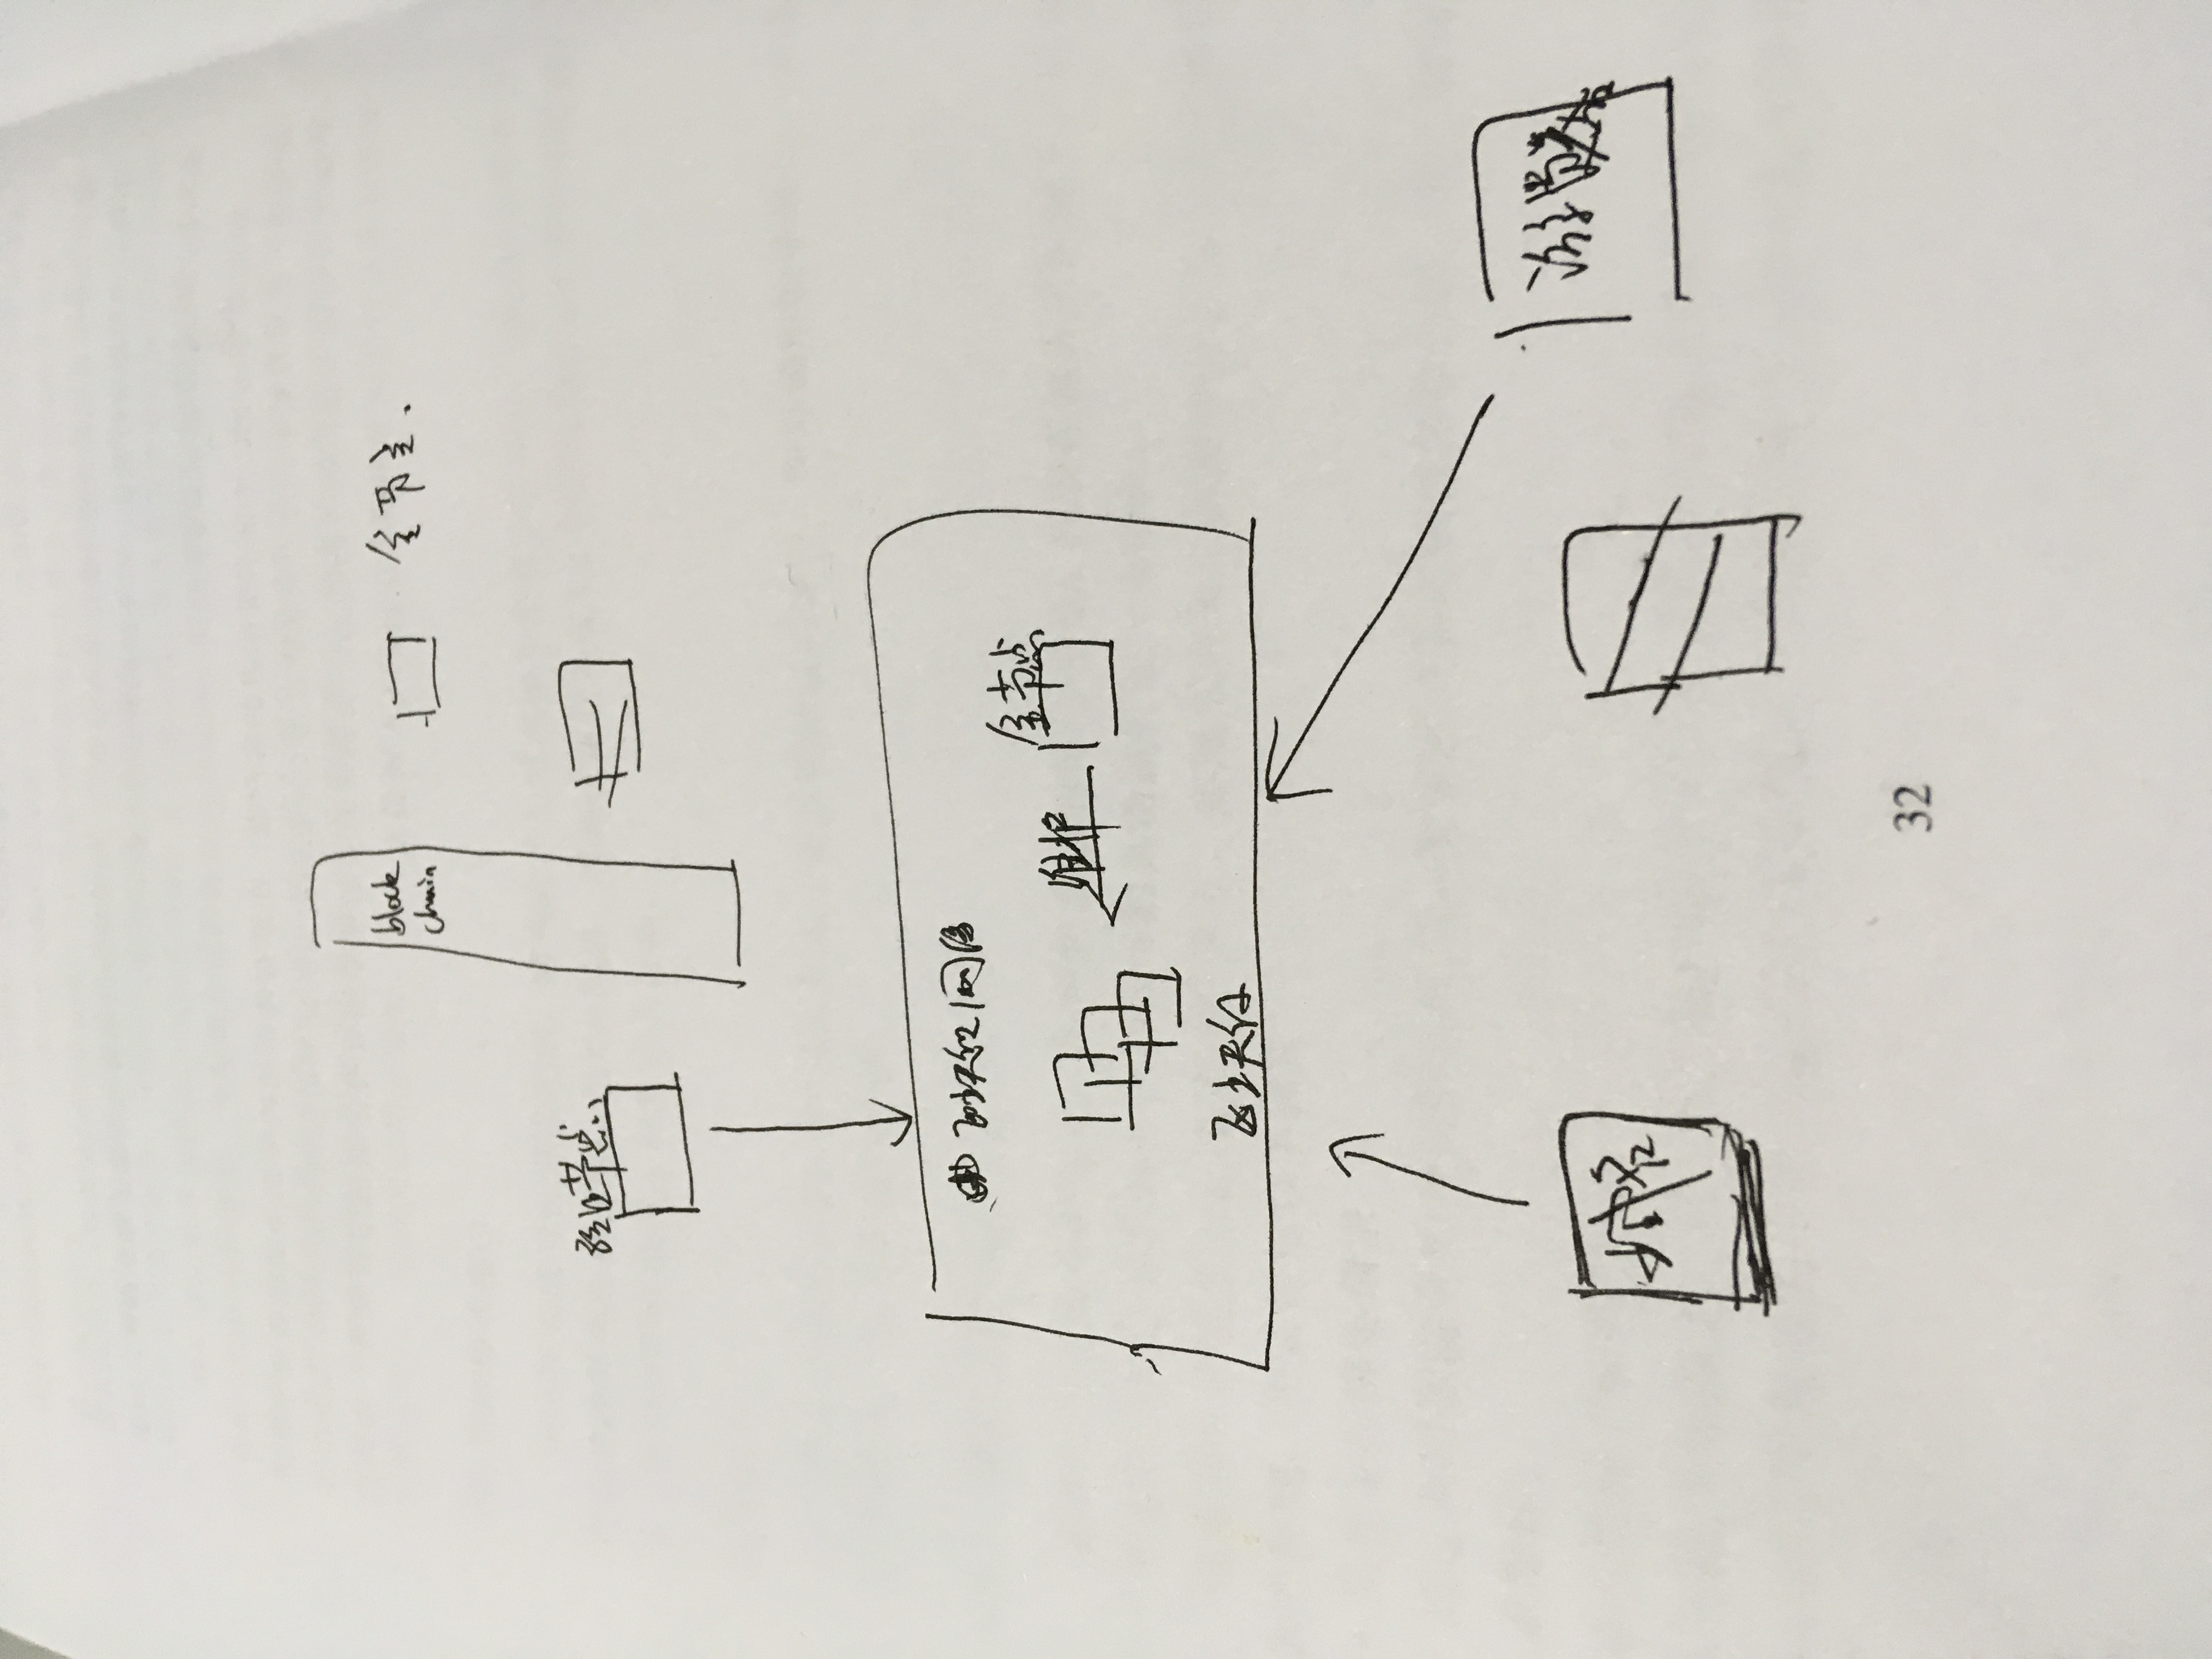
\includegraphics[scale=0.6]{img/system_framework}
 	\caption{系统架构}\label{fig:framework}
\end{figure}



在本系统中,区块链是整个系统的重心,所有参与到系统中的角色都要通过其进行关联。不同的角色之间需要使用不同的工具来完成与区块链网络的交互,依赖方在传统PKI系统中使用的是浏览器来完成对证书的检验,同样,在本系统也依赖与浏览器中的插件来完成对证书的二次验证;对于域名而言,需要有相应的客户端来与区块链进行交互,完成验证请求的发布和相关验证信息的部署;验证节点同样需要有相应的客户端来获取区块链上所提交的验证请求,并通过客户端来判断自己是否能够完成验证请求,对验证请求进行响应;作为维护区块链的全节点,则直接通过区块链的客户端进行区块链维护工作即可。

\subsection{实现方式}

本文所提出的方案是依托于区块链及其上面的用户实体的,所以必须需要一个区块链平台才能完成上述系统的构建,实现本文给出方案。在我看来,实现以上系统有两种方式:一种是利用已有的区块链平台,通过其上的智能合约来完成本文给出方案的相关逻辑和操作;另外一种方式是重新构建一个全新的区块链平台,依据本文中给出方案去设计区块链平台的相关功能和交易,完成上述实体之间的信息交互。

以上提到的两种方式都可以完成本系统的构建,且只是影响该系统中的底层区块链的构建,对上层如域名、依赖方以及验证节点并没有实质性的影响,仅仅是通过不同的方式去访问不同的区块链网络。但是两种不同的实现方式各有利弊额,如表\ref{cmpMethod}所示。

\begin{table}[h] %开始一个表格environment,表格的位置是h,here。   
\begin{tabular}{l*{6}{|c}} %设置了每一列的宽度,强制转换。  
 
\hline  
  & 难度 & 工程量 & 网络建立速度 & 性能 & 独立性 & 全节点维护代价 \\ %用&来分隔单元格的内容 \\表示进入下一行  
\hline %画一个横线,下面的就都是一样了,这里一共有4行内容  
基于智能合约 & 低 & 小 & 快 & 低 & 低 & 高 \\
\hline  
创建新链 & 高 & 大 & 慢 & 高 & 高 & 小 \\
 
\hline  
\end{tabular}  
\caption{实现方式对比}\label{cmpMethod} %显示表格的标题 
\end{table}  

基于智能合约的方式相比于创建新链的方式而言,实现起来可能更加容易,不需要对区块链的底层去进行修改,只需要在上次的智能合约中完成相关功能和模块即可,所以难度更小;同时,基于智能合约的方式只需要将方案转换为智能合约,不需要对区块链的底层进行修改,书写的代码也要少一些,因而工程量更小。由于基于现有的区块链平台去开发智能合约,该平台一般情况下已经积累了一定的用户,很多节点已经在上面进行区块链的维护;而新开发一条链需要一段时间才能有住够多的用户加入到其中,能够保证该系统在创建初始就可以安全有效的进行下去,就系统建立的速度而言,基于智能合约方式更加高效。

但是,基于智能合约的方式也存在着相应的缺点,主要表现在性能、健壮性和全节点付出的代价。由于现有支持智能合约的公链性能都很低,并且其上还充斥这其它智能合约的交易,所以在其上开发智能合约会直接导致本系统的请求处理并不会那么及时,性能会比较低下;而创建一条新链,这可以通过一系列优化来提高其性能。另外一个问题就是整个系统的独立性并不好,很大程度上要取决于依赖的区块链平台,如果该平台出现任何问题,那么将直接影响到本系统的正常工作;最后是全节点付出的代价问题,如果一个全节点想维护本系统中的账本,那么其必须要将该区块链上的所有交易记录都维护下来,包含了一些其它不是很相关的交易,大大提高了其加入本系统的代价。

本文将选择基于智能合约的方式实现,基于的区块链平台为以太坊,身份验证方案选择基于验证次数的方案。



\section{模块设计}
%每个模块都画一个图,写清楚介入数据以及返回数据内容



本方案以区块链作为底层架构,需要在其上需要上述方案中的相关逻辑,让PKI中的相关实体与区块链进行交互,在其上完成身份认证并进行相关数据的存储,实现对域名可信CA列表的访问与控制,并最终完成证书有效性的进一步确认。

根据上一小节的论述,本文中的实现将基于以太坊来完成,在智能合约中编码方案中的相关逻辑。在本小节中,我们将给出系统实现的相关模块,并对模块的功能和实现细节进行描述。我们知道,在本系统中进行信息交互的实体包括域名、验证节点、依赖方以及区块链上的全节点;依据在前面对这些实体的相关功能描述,本系统如\ref{fig:module}图包含四个模块进行实现:智能合约、域名客户端、验证节点客户端、浏览器验证插件。

\begin{figure}[htbp]
 	\centering
 	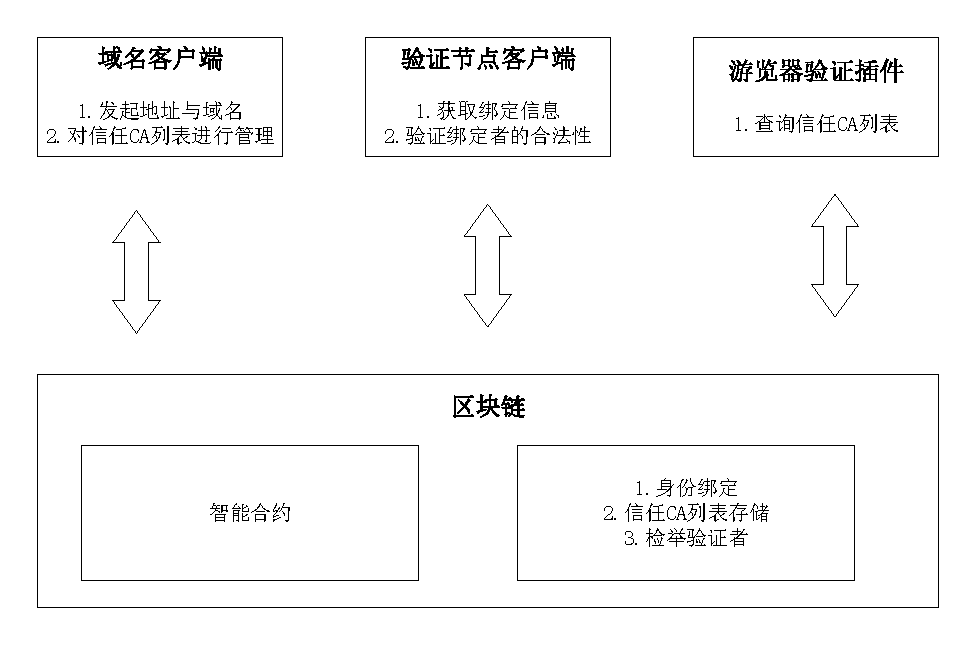
\includegraphics[width = 0.8\textwidth]{img/module}
 	\caption{系统模块设计}\label{fig:module}
\end{figure}


\subsection{智能合约}

\subsubsection{模块功能}

本系统中的所有实体都需要通过区块链进行连接,而在本文的实现方式中,所有的数据都要通过智能合约来完成交互。在智能合约中,不仅要完成对域名信任CA的相关信息存储,还需要完成域名认证的操作,同时,还要向其他的实体提供查询操作。智能合约整个模块需要提供给的功能如下:

\begin{itemize}
	\item 
	\noindent\text{域名认证}

	域名认证功能的服务对象是域名,其作用是让域名可以在区块链网络中完成身份的绑定。该功能中的参与者不仅仅包括域名本身,还包括本系统中的验证节点。当域名调用该功能的时候,将通过在上一章节中设计的验证节点选取方法,选取一系列验证节点来完成验证;在验证信息存在错误的时候,本系统的中其它节点还可以对认证过程发起检举,并通过相关的机制来完成对检举确认。

	\item 
	\noindent\text{信任列表存储}

	信任列表存储是该模块中的另外一个功能,其面向的对象是已经通过身份验证的域名节点,通过本功能可以更改智能合约中存储的数据,完成对自身可信CA的控制。

	\item
	\noindent\text{信任列表查询}

	信任列表查询功能面向的对象是PKI系统中的依赖方,通过该功能完成对特定域名可信CA列表的查询。

\end{itemize}


\subsubsection{模块接口}

根据智能合约模块的功能知道,本模块需要接收域名的认证请求、验证节点的验证信息和检举信息以及域名对信任CA列表的修改、其它实体对信任CA列表的查询,本模块需要提供的接口如表\ref{table:smartContractInterface}所示。

\begin{table}[h] %开始一个表格environment,表格的位置是h,here。   
\centering
\begin{tabular}{p{3.2cm}|p{2cm}|p{2.5cm}|p{2cm}|p{4cm}} %设置了每一列的宽度,强制转换。  
\hline  
 接口名称 & 面向对象 & 参数 & 返回值 & 接口功能\\ %用&来分隔单元格的内容 \\表示进入下一行  
\hline
register & 域名 & 绑定地址、域名名称 & 无 & 发起身份绑定请求 \\
\hline 
report & 验证节点 & 域名绑定地址、域名名称 & 无 & 发起绑定检举 \\
\hline 
verify & 验证节点 & 待绑定地址、域名名称、验证内容 & 无 & 发起验证确认 \\
\hline 
modifyTrustedCAs & 域名 & 域名名称、可信CA列表 & 无 & 修改域名自身的可信CA列表 \\
\hline 
queryTrustedCAs & 任意实体 & 域名名称 & 可信CA列表 & 查询给定域名的可信CA列表 \\
\hline 
\end{tabular}  
\caption{智能合约接口设计}\label{table:smartContractInterface} %显示表格的标题 
\end{table} 

% 通过以上接口,本系统中的角色与区块链进行交互,完成信息的获取和修改。


% \begin{itemize}
% 	\item 
% 	\noindent\text{认证请求接口}
% 	%面向对象,需要提交内容,返回信息,达到什么样的目的。

% 	该接口面向的对象为域名,调用需要提供的数据包括自身的公钥和域名。

% 	\item
% 	\noindent\text{检举接口}

% 	该接口面向的对象为验证节点,调用需要提供的数据包括自身的公钥和检举绑定的公钥和域名。

% 	\item
% 	\noindent\text{验证接口}

% 	该接口面向的对象为验证节点,调用该接口前需要获取验证者在网络中放置的验证信息,并且需要在本地产生一个相应的用户证明,提交的内容包括验证信息、自身公钥和用户证明。

% 	\item
% 	\noindent\text{信任列表修改接口}

% 	该接口面向的对象为通过验证的域名,调用该接口需要提供自身的公钥和相应的信任CA列表。

% 	\item
% 	\noindent\text{信任列表查询接口}

% 	该接口面向的对象为依赖方,调用该接口需要提供查询的域名地址,将会返回该域名对应的信任CA列表。
	

% \end{itemize}




\subsection{域名客户端}

\subsubsection{模块功能}

域名作为证书的申请者,需要将自己的可信任CA列表存储到区块链上,以供证书受用者在使用证书的过程中对证书的真伪进行进一步检查。

域名客户端需要与区块链进行交互,实现域名和公钥的绑定以及对自己可信CA列表的控制,该模块包括的功能如下:

\begin{itemize}
	\item 
	\noindent\text{密钥管理}

	区块链上的身份是通过公私钥对来完成控制的,所以在该模块中,需要提供密钥管理功能来对区块链上的身份进行管理。其中包括密钥的生成和保存,其中公钥将作为本系统中的地址;其次是需要在必要的时候使用私钥完成签名操作,包括对交易的签名和验证信息的签名。

	\item 
	\noindent\text{发起认证请求}

	客户端的另外一个重要功能就是发起认证请求,向区块链网络公布自己拥有的域名和响应的密钥。在区块链对请求进行纳入后,根据交易生成相关的验证内容。

	\item
	\noindent\text{修改信任列表}

	信任列表的修改功能是在域名完成认证后才可使用的功能,向区块链网络提交自己的信任CA列表,供网络中搞定其它节点查询。

\end{itemize}

\subsubsection{模块逻辑}

域名客户端模块需要完成以上功能,为了能够对自身信任列表的控制,其模块运行逻辑如图\ref{fig:domaincli_work_flow}所示。

\begin{figure}[htbp]
 	\centering
 	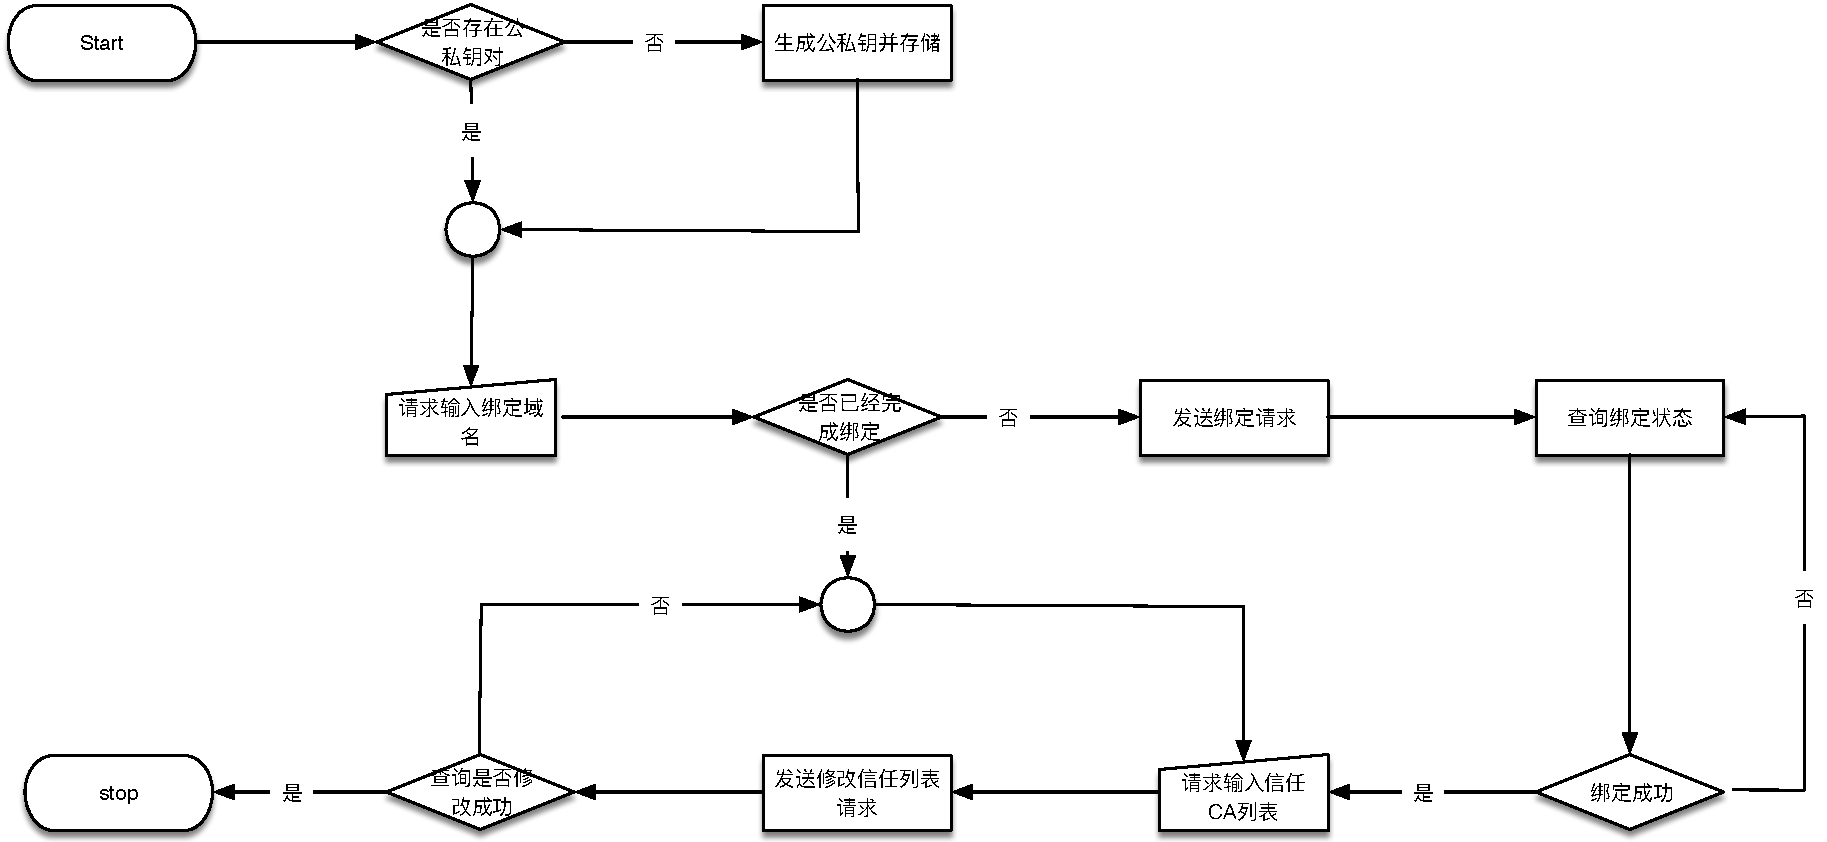
\includegraphics[width=1\textwidth]{img/domaincli_work_flow}
 	\caption{域名客户端模块流程}\label{fig:domaincli_work_flow}
\end{figure}




\subsection{验证节点客户端}

\subsubsection{模块功能}

验证节点是本系统中身份鉴权的重要组成部分,是身份绑定有效性的保证,只有住够多验证节点存在的情况下,才可以保证身份确认的有效。

验证节点的主要工作是实时的查询验证请求并对验证请求进行验证,并根据其验证请求计算自己是否符合验证节点的要求,如果符合的话将进行验证确认操作,如果不是,也可以进行验证,对不符的验证提交检举交易。所以本模块包含的功能如下:

\begin{itemize}
	\item 
	\noindent\text{密钥管理}

	通域名客户端一样,验证节点在区块链上身份是由公私钥来完成控制的,所以同样需要密码管理功能,完成对自身身份的控制。

	\item 
	\noindent\text{请求验证}
	%面向对象,需要提交内容,返回信息,达到什么样的目的。
	验证节点客户端将对区块链上发起的请求进行监控,包括身份绑定请求和检举信息,对所有的请求都会验证,并将验证的结果呈现在客户端中。

	\item
	\noindent\text{请求处理}

	本客户端会对所有的验证请求进行验证,当验证请求通过的且自己能够成为该请求的验证者时,将会发起交易确认,从而获得相应的奖励。当请求存在问题是,如果是绑定请求,那么发送检举交易到区块链上;如果是检举确认,将根据确认情况进行确认。
	

\end{itemize}

\subsubsection{模块逻辑}

验证节点客户端需要实时的获取区块链网络中的绑定请求,并查询相关请求的验证内容,对请求做出回应,本模块的运行逻辑如下如\ref{fig:validator_work_flow}所示。


\begin{figure}[htbp]
 	\centering
 	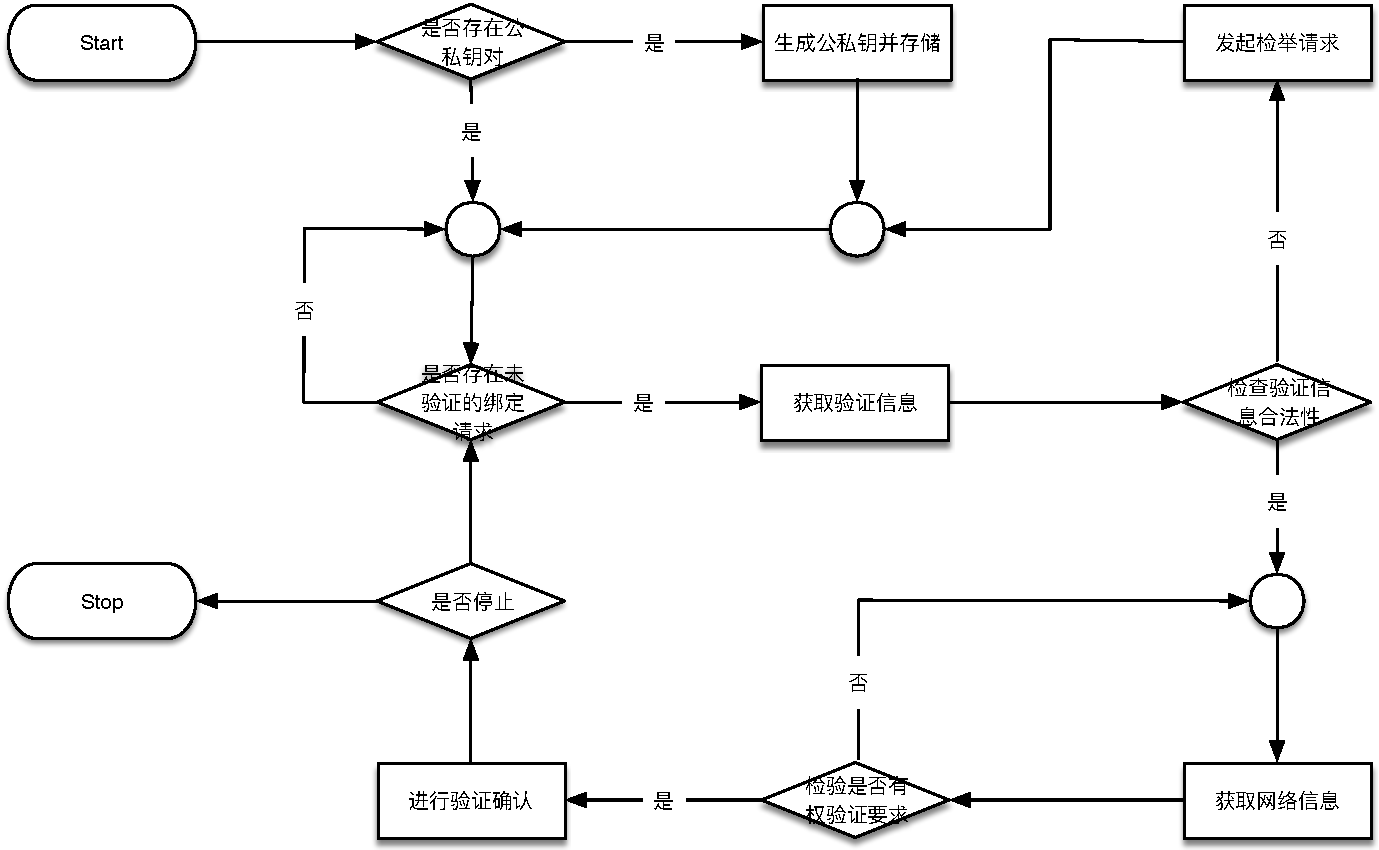
\includegraphics[scale=0.6]{img/validator_work_flow}
 	\caption{验证客户端模块流程}\label{fig:validator_work_flow}
\end{figure}


% \subsubsection{模块接口}

% 根据本模块需要完成的功能,需要完成以下接口:



% \begin{itemize}
% 	\item 
% 	\noindent\text{密钥管理接口}

% 	%面向对象,需要提交内容,返回信息,达到什么样的目的。
% 	用户调用该接口可以实现对密钥的生成、管理和使用,在验证信息生过程中将调用该接口对验证信息进行生成。由于在进行验证过程中需要提供容量证明,所以本接口中还包含了容量证明的初始化操作。

% 	\item
% 	\noindent\text{请求操作接口}

% 	本接口将完成对一个请求的确认,其根据请求的内容,在本地存储的容量证明中得到相关的证明,提交到智能合约模块中的验证接口。如果当一个请求不合法是,将提交否定确定或者检举信息。
	

% \end{itemize}


\subsection{浏览器验证插件}

\subsubsection{模块功能}

浏览器是Web PKI中证书受用者的客户端,在原有体系结构中充当着检查证书真伪的角色。在本方案中,为了保证被恶意CA私自签发的证书可以被识别出来,需要在客户端进行对证书进行额外的检查,也就是需要浏览器需要有区块链进行交互,查询收到的证书是否由证书申请者信任的CA所签发。

本模块相比于前面的模块较为简单,只需要通过调用智能合约中的信任列表查询模块,获取域名可信CA列表与证书进行对比,在发现错误的时候向用户发出警告。

\subsubsection{模块流程}

浏览器验证插件需要在游览器访问网址时获得域名的证书,同时通过智能合约的相关接口获取域名设置的信任CA列表,并与证书签发者对比,具体的流程如图\ref{fig:chrome_extension}所示。

\begin{figure}[htbp]
 	\centering
 	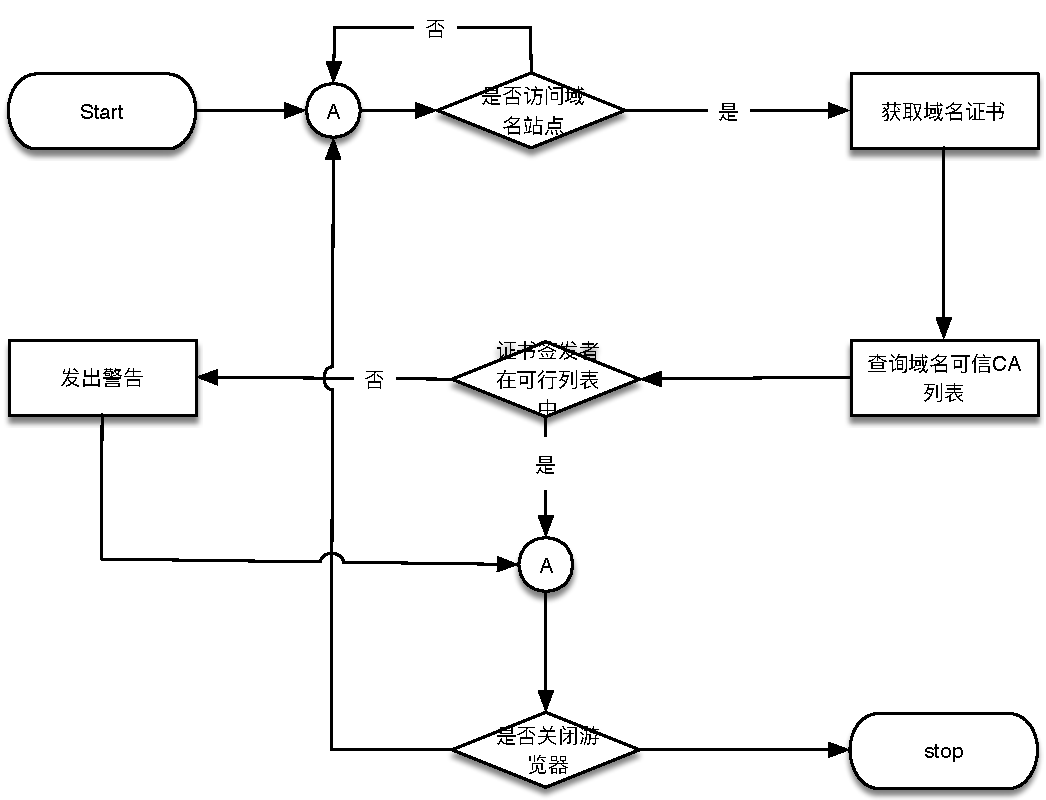
\includegraphics[width=1\textwidth]{img/chrome_extension}
 	\caption{浏览器验证插件模块流程}\label{fig:chrome_extension}
\end{figure}

% 根据本模块相关功能,需要完成以下接口:

% \begin{itemize}
% 	\item 
% 	\noindent\text{获取证书接口}

% 	在依赖方使用浏览器与域名建立通信的过程中,浏览器将收到域名的赠书,本模块需要在完成证书检查前需要通过本接口完成对证书的获取,位后续操作提供基础。

% 	\item
% 	\noindent\text{获取信任CA接口}

% 	在取得域名证书之后,需要获取该域名信任CA列表,已完成证书签发者与之的比较。
	

% \end{itemize}



% vim:ts=4:sw=4

\section{系统测试}


\subsection{环境搭建}



实验所需的区块链网络搭建在阿里云服务中,如图\ref{fig:platform}所示。区块链网络中包含5台阿里云服务器,作为全节点完成对区块链网络的维护;另外5台服务器作为验证节点,每台服务器上启动10个验证客户端,共计拥有50个验证节点;1台阿里云部署web服务,作为域名服务器并运行域名客户端;本地PC作为依赖方,模拟完成对域名的访问,在过程中完成对信任CA列表的获取。

\begin{figure}[htbp]
 	\centering
 	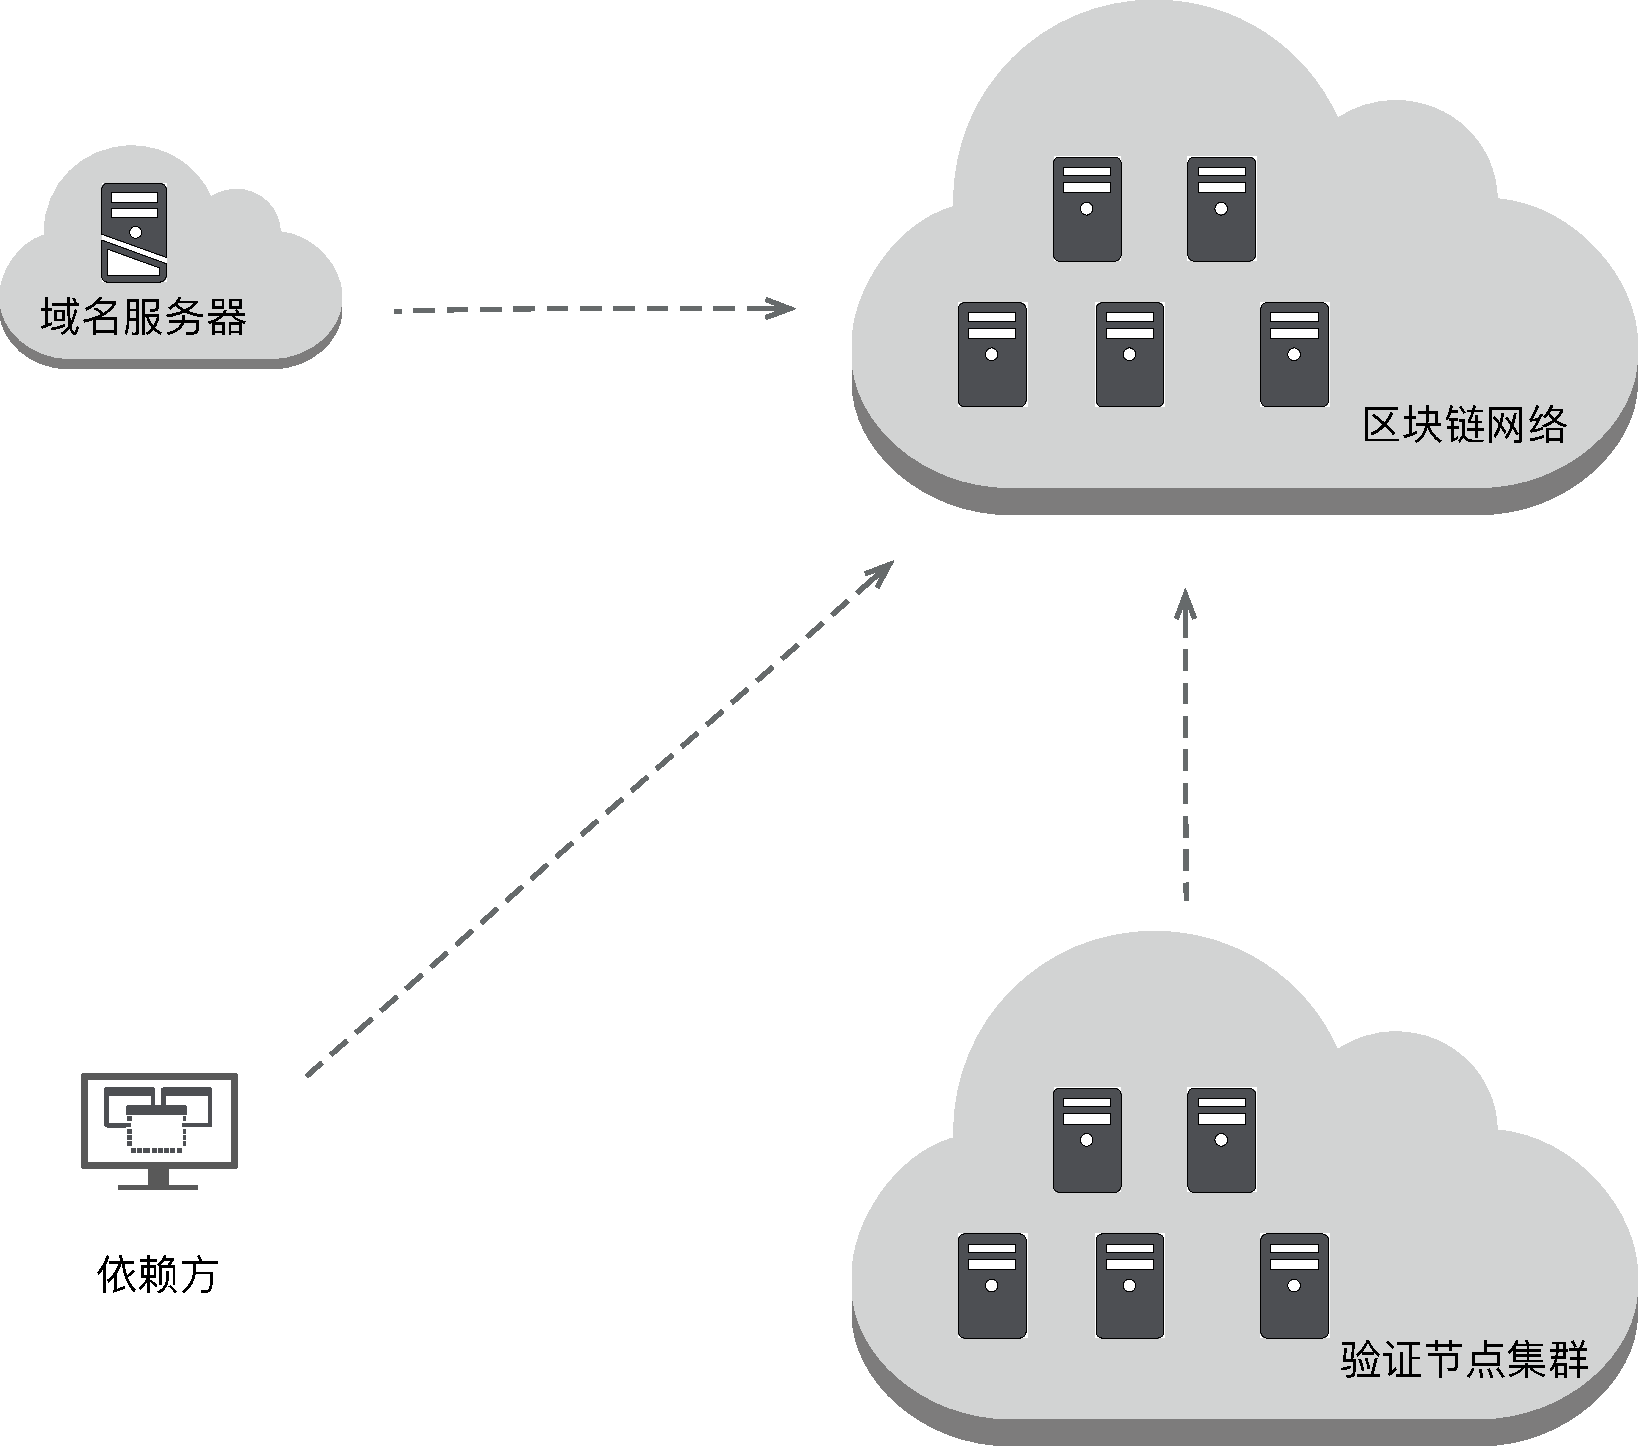
\includegraphics[scale = 0.4]{img/platform}
 	\caption{平台搭建}\label{fig:platform}
\end{figure}

阿里云服务器配置如下:

\begin{itemize}
	\item CPU: 1核
	\item 操作系统: Ubuntu 16.04(64 bit)
	\item 内存: 2GB
	\item 磁盘: 40GB
	\item Golang: 1.8.3
	\item Ethereum: Titanium(v1.8.7)
\end{itemize}

本机配置如下:
\begin{itemize}
	\item CPU: 8核
	\item 操作系统: macOs High Sierra(version 10.13.3)
	\item Chrome: Version 66.0.3359.139(64-bit)
\end{itemize}

%参数选择和设置

\subsection{相关参数}

本系统实现的认证方案是基于验证次数的方案,在该方案中将涉及到一些参数的设置,如表\ref{table:param}所示。



\begin{table}[h] %开始一个表格environment,表格的位置是h,here。   
\centering
\begin{tabular}{l*{3}{|p{2cm}}*{2}{|p{3cm}}} %设置了每一列的宽度,强制转换。  
\hline  
 参数符号 & $n$ &  $d$ & $t_{adjust}$ & $Info_{rcvBlock}$ & $Info_{curBlcok}$ \\ %用&来分隔单元格的内容 \\表示进入下一行  
\hline %画一个横线,下面的就都是一样了,这里一共有4行内容  
 数值 & 10 & 1 & 1(/块)  & Block Hash & Block num\\
\hline  
 参数含义 & 身份绑定需要10次确认 & 初始海明距离为1 & 每隔1块调整一次挑选验证节点准则 & 接收交易的区块信息为所在区块的哈希值& 当前区块的信息为该区块的编号  \\
\hline 
\end{tabular}  
\caption{参数设置及含义}\label{table:param} %显示表格的标题 
\end{table} 

% \subsection{模块实现}
% \subsubsection{智能合约}
% \subsubsection{验证客户端}
% \subsubsection{域名客户端}
% \subsubsection{浏览器验证插件}

\subsection{功能测试}

本小节对系统实现进行简要测试,依据系统的部署和正常调用流程,检验系统实现的正确性。具体流程如下:

%可能给出不同节点加入验证完成时间

\noindent\textbf{1. 智能合约部署}

在智能合约开发和部署过程中,使用truffle工具来进行;在完成开发工作后,通过设置truffle工程目录下的truffle.js文件设置连接区块链网络节点ip和端口,然后使用compile和migrate命令来完成对智能合约的部署。在连接节点上可以看到以下日志:

\begin{lstlisting}[caption={智能合约部署日志}, label=code:deploy]
[9:45:59 AM] eth_sendTransaction
[9:46:00 AM]   Transaction: 0x6fde67cd2a4419468b0764df675bad9ded7d64358dae8373410a73bb128490cf
[9:46:00 AM]   Contract created: 0x4e60d62f8dee99d577fa8248843f0c49e4244662
[9:46:00 AM]   Gas usage: 1135286
[9:46:00 AM]   Block Number: 1
[9:46:00 AM]   Block Time: Sun May 06 2018 09:55:59 GMT+0800 (CST)

\end{lstlisting}

\noindent\textbf{2. 认证接口调用}

在域名客户端配置智能合约地址$0x4e60d62f8dee99d577fa8248843f0c49e4244662$,以及需要连接的区块链节点ip和端口;运行一下命令,发起验证请求服务:

\begin{lstlisting}
domain-cli reg 0x67ec76ad62a83a32ece695d5f7e9580c2e625b80 www.baidu.com
\end{lstlisting}

得到以下输出:

\begin{lstlisting}

2018-05-09 09:48:31,351 :16 - domain-cli - sending the register request...
2018-05-09 09:48:31,421 :18 - domain-cli - {'status': 'added', 'txn_receipt': AttributeDict({'transactionHash': HexBytes('0xf5e7d6b5a51e7279ed8917d88d0a36aa1174856094c5ac7b4c39d82054d05816'), 'transactionIndex': 0, 'blockHash': HexBytes('0x971344c24a7801b1645c47f885c27e258effbae5f1c20c45a2505237aa13dce2'), 'blockNumber': 2, 'gasUsed': 189579, 'cumulativeGasUsed': 189579, 'contractAddress': None, 'logs': [], 'status': 1, 'logsBloom': HexBytes('0x..0')})}
2018-05-09 09:48:31,421 :22 - domain-cli - The request have been accepted!
2018-05-09 09:48:31,421 :24 - domain-cli - waitting for register completed...
2018-05-09 09:48:31,553 :32 - domain-cli - register completed!
2018-05-09 09:48:31,554 :42 - domain-cli - please put 3575248931332620452 atwww.baidu.com/1851786109301171516.
2018-05-09 09:48:31,590 :48 - domain-cli - waiting validator to complete authorization (0/10)
...
2018-05-09 09:50:32,660 :48 - domain-cli - waiting validator to complete authorization (9/10)
2018-05-09 09:50:37,695 :48 - domain-cli - waiting validator to complete authorization (10/10)
2018-05-09 09:50:37,695 :50 - domain-cli - authorization completed!
 \end{lstlisting}

\noindent\textbf{3. 验证请求调用}

在域名客户端配置智能合约地址$'0x4e60d62f8dee99d577fa8248843f0c49e4244662'$,以及需要连接的区块链节点ip和端口;通过对区块链的监控,当域名exmaple.com发起验证时,将运行validator-cli程序将自动发起验证,得到以下日志:

\begin{lstlisting}

2018-05-09 09:48:50,488 :11 - validator-cli - check new authorization request...
2018-05-09 09:48:50,573 :21 - validator-cli - get vcode 3575248931332620452 from www.baidu.com/1851786109301171516.
2018-05-09 09:48:50,573 :23 - validator-cli - the vcode is right, check passed!
2018-05-09 09:48:50,573 :26 - validator-cli - waiting for new block to confirm this request...
...
2018-05-09 09:48:50,574 :26 - validator-cli - waiting for new block to confirm this request...
2018-05-09 09:48:50,574 :28 - validator-cli - ready to confirm :)
2018-05-09 09:48:50,574 :29 - validator-cli - sending confirmation requset...
2018-05-09 09:48:50,630 :31 - validator-cli - {'status': 'added', 'txn_receipt': AttributeDict({'transactionHash': HexBytes('0xab0bcf480e2f9906aaa9c70675158236d6e912931759b768eb0d025a5e0c20d7'), 'transactionIndex': 0, 'blockHash': HexBytes('0x1a01ec45298e0167e158ef4bea077a2e0448ffdb144377f286ed4b8ff4f3c77a'), 'blockNumber': 3, 'gasUsed': 107323, 'cumulativeGasUsed': 107323, 'contractAddress': None, 'logs': [], 'status': 1, 'logsBloom': HexBytes('0x0..0')})}
2018-05-09 09:48:50,630 :37 - validator-cli - confirmation request sent successfully.

\end{lstlisting}


\noindent\textbf{4. 信任列表修改}

在域名客户端运行domain-cli query 命令查询验证请求状态;待绑定完成后,通过一下来修改信任CA列表:

\begin{lstlisting}
domain-cli modifyTrustedCAs "Symantec Corporation" 
\end{lstlisting}


得到如下输出:

\begin{lstlisting}
2018-05-09 09:50:37,750 :56 - domain-cli - Sending modify Trusted CAs request...
2018-05-09 09:50:37,750 :59 - domain-cli - {'status': 'added', 'txn_receipt': AttributeDict({'transactionHash': HexBytes('0x7b39338a2d30624e339eb4b3261efa5fa09378936d2cad07c17fd5406ae40729'), 'transactionIndex': 0, 'blockHash': HexBytes('0x31a3306ce2fa4e09a9eafc5eaa3a0cf910f69b87d6c93271a2ce0df0f26b955f'), 'blockNumber': 14, 'gasUsed': 46593, 'cumulativeGasUsed': 46593, 'contractAddress': None, 'logs': [], 'status': 1, 'logsBloom': HexBytes('0x0...0')})}
2018-05-09 09:50:37,750 :63 - domain-cli - trusted CAs be modified to Symantec Corporation
\end{lstlisting}

\noindent\textbf{5. 信任列表查询}

在前面的操作中,我们将www.baidu.com的信任CA设置为了Symantec Corporation,和其正在使用的证书签发机构是一致的。在游览器端安装chrome插件之后,访问www.baidu.com,插件显示内容如图\ref{fig:pass}所示。

\begin{figure}[htbp]
 	\centering
 	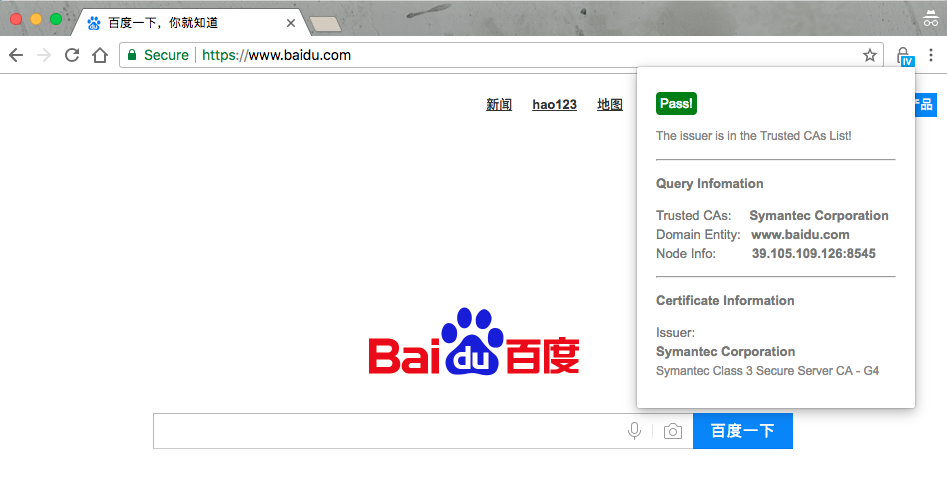
\includegraphics[scale=0.3]{img/pass}
 	\caption{验证通过实例}\label{fig:pass}
\end{figure}

在上图中,第一行表示是否通过验证,本例中通过验证;第二行表示设置的信任CA,后面内容为证书相关的信息。


由于没有对www.google.com进行绑定操作,将无法查询得到信任CA列表,所以其无法通过验证,得到结果如图\ref{fig:notPass}所示。

\begin{figure}[htbp]
 	\centering
 	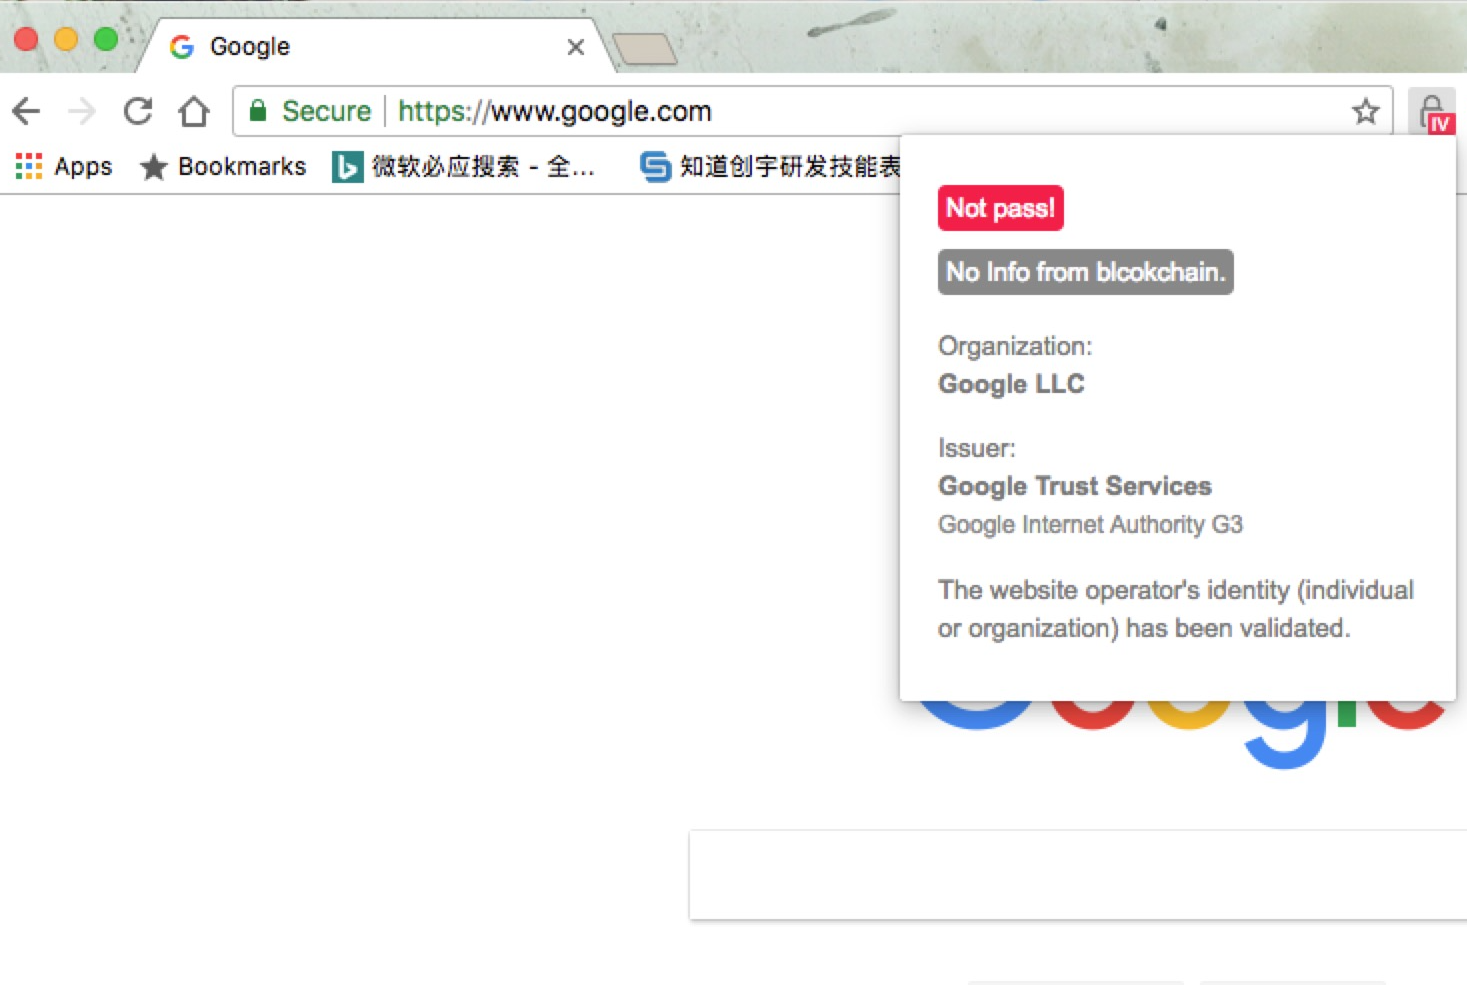
\includegraphics[scale=0.3]{img/notPass}
 	\caption{验证未通过实例}\label{fig:notPass}
\end{figure}


通过以上测试可以知道,通过实现的系统可以正常完成域名的身份认证已经信任CA列表的绑定;并且通过游览器插件,在访问网页是可以获得相关的验证结果。

% \subsubsection{智能合约部署}

% \subsubsection{域名客户端发起认证请求}

% \subsubsection{验证节点客户端进行身份确认}

% \subsubsection{域名客户端进行信任CA列表修改}

% \subsubsection{游览器发起网页请求}



